\chapter{Risultati\label{sec:risultati}}
\noindent In questa sezione mostriamo i risultati ottenuti dall'algoritmo, ovvero i tempi medi impiegati per full contraction e karger, il discovery time, la soluzione trovata, la soluzione attesa e l'errore relativo.

\section{Grafici\label{sec:grafici}}

\subsection{Full contraction\label{sec:fc}}
\begin{figure}[htp]
    \centering
    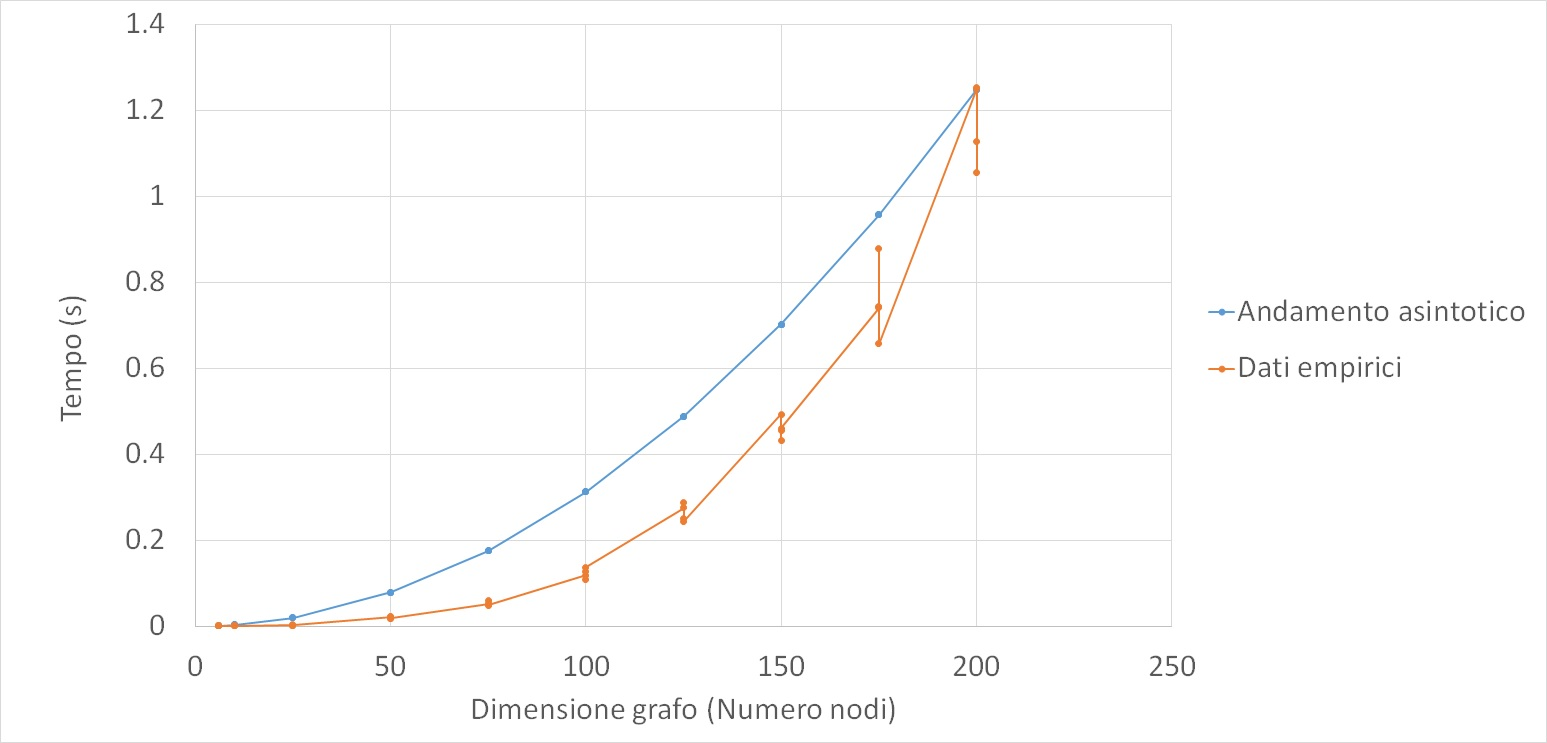
\includegraphics[width=\textwidth]{immagini/full_contraction.jpg}
\end{figure}
Il presente grafico illustra i tempi di calcolo della procedura Full\_Contraction sui grafi del dataset al variare del numero di vertici. Confrontiamo con la complessità asintotica stimata di \(O(n^{2})\).

\subsection{Karger\label{sec:karger}}
\begin{figure}[htp]
    \centering
    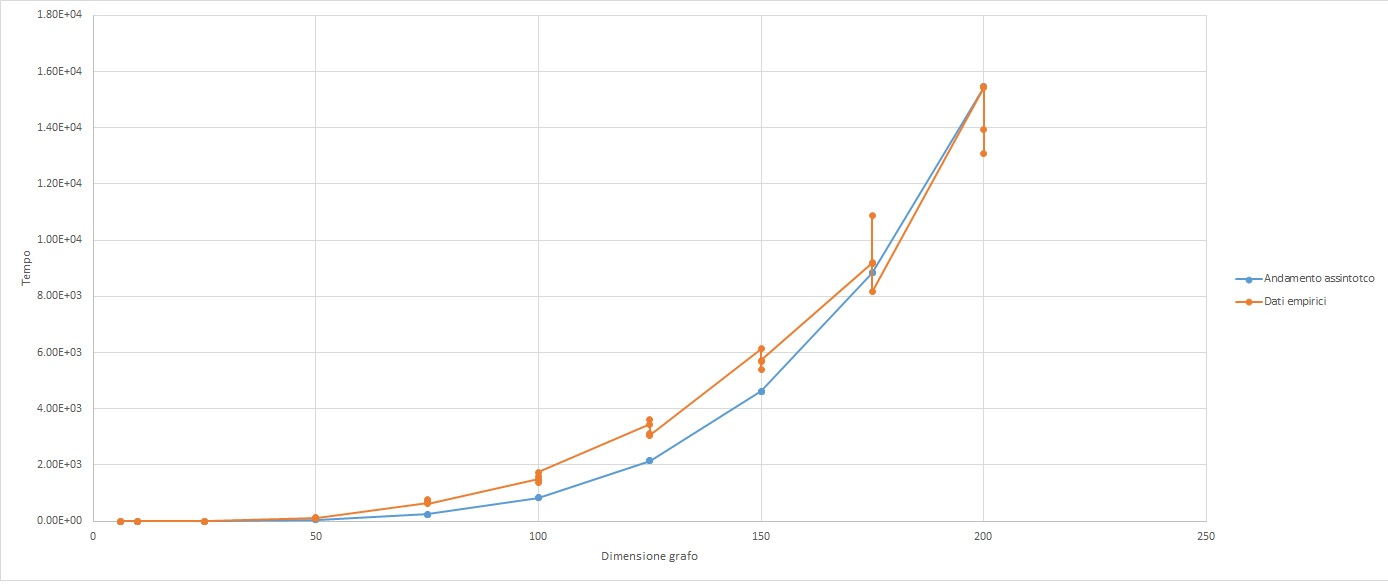
\includegraphics[width=\textwidth]{immagini/karger.jpg}
\end{figure}
Il presente grafico illustra i tempi di calcolo dell'algoritmo di Karger sui grafi del dataset al variare del numero di vertici. La probabilità di errore è uguale a \(\frac{1}{n}\) di sbagliare per grafi inferiori a $75$ nodi. Tale scelta è dovuta a motivi di tempo, come illustrato in sezione \vref{sec:originalita}. Confrontiamo con la complessità asintotica stimata di \(O(n^{4}log(n))\).


\section{Tabella\label{sec:tabella}}

\footnotesize
\begin{tabularx}{\textwidth}{*{10}{Y}}
    \toprule
    \textbf{Istanza} & \textbf{Tempo di una Full contraction (s)} & \textbf{Discovery time (s)} & \textbf{Tempo totale (s)} & \textbf{Soluzione trovata} & \textbf{Soluzione ottimo} & \textbf{Errore relativo}\\
    \endfirsthead
    \toprule
    \textbf{Istanza} & \textbf{Tempo di una Full contraction (s)} & \textbf{Discovery time (s)} & \textbf{Tempo totale (s)} & \textbf{Soluzione trovata} & \textbf{Soluzione ottimo} & \textbf{Errore relativo}\\
    \endhead
    \midrule
    input\_01\_6	&	0.00006420	&	0.00131726	&	0.00717187	&	2	&	2	&	0.0	\\\midrule
	input\_02\_6	&	0.00006785	&	0.00022292	&	0.03581977	&	1	&	1	&	0.0	\\\midrule
	input\_03\_6	&	0.00007611	&	0.00034499	&	0.00778651	&	3	&	3	&	0.0	\\\midrule
	input\_04\_6	&	0.00007507	&	0.00027013	&	0.00872898	&	4	&	4	&	0.0	\\\midrule
	input\_05\_10	&	0.00019939	&	0.00230646	&	0.05261183	&	4	&	4	&	0.0	\\\midrule
	input\_06\_10	&	0.00016412	&	0.00085616	&	0.04731894	&	3	&	3	&	0.0	\\\midrule
	input\_07\_10	&	0.00017446	&	0.00273633	&	0.04886866	&	2	&	2	&	0.0	\\\midrule
	input\_08\_10	&	0.00017658	&	0.00046015	&	0.04921460	&	1	&	1	&	0.0	\\\midrule
	input\_09\_25	&	0.00198467	&	0,00161695	&	2.71520424	&	7	&	7	&	0.0	\\\midrule
	input\_10\_25	&	0.00181535	&	0.36311722	&	2.52611518	&	6	&	6	&	0.0	\\\midrule
	input\_11\_25	&	0.00202685	&	0.01288033	&	2.87397146	&	8	&	8	&	0.0	\\\midrule
	input\_12\_25	&	0.00285040	&	0.59262013	&	3.88847303	&	9	&	9	&	0.0	\\\midrule
	input\_13\_50	&	0.02205332	&	1.16963172	&	119.23173952	&	15	&	15	 & 0.0	\\\midrule
	input\_14\_50	&	0.02155554	&	0.60323572	&	115.70873451	&	16	&	16	 & 0.0	\\\midrule
	input\_15\_50	&	0.01671049	&	2.41417027	&	91.38596511		&	14	&	14	 & 0.0	\\\midrule
	input\_16\_50	&	0.01808762	&	1.16370130	&	98.28982854		&	10	&	10	 & 0.0	\\\midrule
	input\_17\_75	&	0.05015093	&	7.60165477	&	651.79445624	&	19	&	19	 & 0.0	\\\midrule
	input\_18\_75	&	0.05971390	&	2.65774322	&	769.72895575	&	15	&	15	 & 0.0	\\\midrule
	input\_19\_75	&	0.05304535	&	0.42174196	&	687.63417149	&	18	&	18	 & 0.0	\\\midrule
	input\_20\_75	&	0.04822129	&	0.92826390	&	628.02836180	&	16	&	16	 & 0.0	\\\midrule
	input\_21\_100	&	0.11767139	&	0.41041040	&	1496.49857569	&	22	&	22 & 0.0	\\\midrule
	input\_22\_100	&	0.10784917	&	24.04785800	&	1376.93518615	&	23	&	23 & 0.0	\\\midrule
	input\_23\_100	&	0.12643225	&	2.35784650	&	1606.15633321	&	19	&	19 & 0.0	\\\midrule
	input\_24\_100	&	0.13665407	&	32.93737745	&	1735.68474460	&	24	&	24 & 0.0	\\\midrule
	input\_25\_125	&	0.27526138	&	10.41306686	&	3446.43969345	&	34	&	34 & 0.0	\\\midrule
	input\_26\_125	&	0.24957255	&	8.42978859	&	3130.82415271	&	29	&	29 & 0.0	\\\midrule
	input\_27\_125	&	0.28772694	&	69.54419684	&	3600.48817873	&	36	&	36 & 0.0	\\\midrule
	input\_28\_125	&	0.24376734	&	12.67581010	&	3059.99670696	&	31	&	31 & 0.0	\\\midrule
	input\_29\_150	&	0.49271837	&	35.33633661	&	6129.14617682	&	37	&	37 & 0.0	\\\midrule
	input\_30\_150	&	0.45532591	&	83.78166389	&	5669.51948738	&	35	&	35 & 0.0	\\\midrule
	input\_31\_150	&	0.43285431	&	32.14746523	&	5394.68515444	&	41	&	41 & 0.0	\\\midrule
	input\_32\_150	&	0.45989296	&	58.75906992	&	5726.16600871	&	39	&	39 & 0.0	\\\midrule
	input\_33\_175	&	0.74070684	&	66.79247236	&	9177.23712540	&	42	&	42 & 0.0	\\\midrule
	input\_34\_175	&	0.74288779	&	49.13439870	&	9205.83131051	&	45	&	45 & 0.0	\\\midrule
	input\_35\_175	&	0.87808876	&	45.06704497	&	10859.42819190	&	53	&	53 & 0.0	\\\midrule
	input\_36\_175	&	0.65710520	&	6.00958300	&	8155.21835065	&	43	&	43 & 0.0	\\\midrule
	input\_37\_200	&	1.25286142	&	20.91466975	&	15461.59397507	&	54	&	54 & 0.0	\\\midrule
	input\_38\_200	&	1.05687901	&	163.0276653	&	13067.47582197	&	52	&	52 & 0.0	\\\midrule
	input\_39\_200	&	1.12854942	&	13.06262207	&	13932.64299393	&	51	&	51 & 0.0	\\\midrule
	input\_40\_200	&	1.25152820	&	93.24242926	&	15435.27277613	&	61	&	61 & 0.0 \\\bottomrule
    \caption{Risultati}\label{tab:risultati}
\end{tabularx}

\normalsize